%
% Chapter 5 - Frontend
%
\chapter{Frontend} \label{cap:frontend}

This chapter describes the frontend implementation of EduCal: how the codebase is organized, how it communicates with the backend, and every screen and dialog that makes up the application.

\section{Structural Organization} \label{sec:frontend-organization}

EduCal is a single Next.js application (App Router) that hosts both frontend and backend, rather than two separate projects. The \texttt{app/} directory is kept as a thin routing layer (the calendar home page, the login page, the admin users page, and the API route handlers under \texttt{app/api/}), while the actual UI is organized by feature under \texttt{features/}: \texttt{features/calendar/} (the calendar itself, including views, dialogs, header controls, drag-and-drop, and settings), \texttt{features/auth/} (the login form), and \texttt{features/admin-users/} (the user management dashboard). Reusable, feature-agnostic UI primitives (buttons, dialogs, forms, selects, etc.) live under \texttt{components/ui/}, sourced and adapted from \textbf{shadcn/ui} rather than installed as a compiled dependency, and code shared between client and server (types, Zod schemas, role logic) lives under \texttt{shared/}.

\section{API Communication Architecture} \label{sec:frontend-api}

EduCal deliberately does not use HTTP API routes for reading data. Server components fetch data directly by calling backend services: \texttt{features/calendar/requests.ts}, marked \texttt{"server-only"}, is invoked once from the \texttt{Calendar} server component, and the result (events, users, enum values, vacations) is passed down as initial props into a React context provider (\texttt{CalendarProvider}), avoiding a network round-trip for the common case of simply loading the calendar.

Mutations (creating or editing an event, logging in, managing users) do go through HTTP: a shared fetch wrapper (\texttt{lib/api-client.ts}) attaches the JSON content type, unwraps the \texttt{\{ data: ... \}} envelope on success, and on failure parses the backend's error envelope (Chapter~\ref{cap:backend}) into a user-facing, translated error message. Feature-specific request modules build on this wrapper per mutation endpoint. Components call these functions inside a try/catch and surface the result as a \texttt{sonner} toast, giving immediate feedback without a full page reload.

\section{Web Application} \label{sec:frontend-web-app}

This section walks through the application as a signed-in user experiences it: how routes are protected, how a session is established, and every screen, dialog, and persistent UI element (such as the notification bell, Section~\ref{sec:frontend-notifications}) that makes up the calendar itself.

\subsection{Navigation and Access Control} \label{sec:frontend-navigation}
The application has three main routes: the calendar (\texttt{/}), the login page (\texttt{/login}), and the admin users page (\texttt{/admin/users}). Route-level access control is handled entirely on the server, in the page component itself, rather than by a client-side auth context: \texttt{app/page.tsx} resolves the current session and redirects to \texttt{/login} if none exists, before any calendar markup is ever sent to the client; \texttt{app/login/page.tsx} redirects an already-authenticated user straight to \texttt{/}; and \texttt{app/admin/users/page.tsx} redirects to \texttt{/login} if unauthenticated and to \texttt{/} if the current user is not an \texttt{admin}. On the calendar page, once the session check passes, the actual event/user/enum/vacation data is fetched inside the \texttt{Calendar} component behind a \texttt{Suspense} boundary, which shows a loading skeleton while it resolves.

\subsection{Notification Bell} \label{sec:frontend-notifications}
Once authenticated, every page shows a bell icon in the global navbar, backed by the notification system described in Section~\ref{sec:backend-notifications}. \texttt{NotificationBell} polls \texttt{GET /api/notifications} every 60 seconds and keeps an unread-count badge on the icon; opening it lists each unread notification's occurrence description and date, with a ``mark all read'' shortcut. Clicking one marks it read and navigates to \texttt{/?openEventId=\ldots\&openOccurrenceId=\ldots}; \texttt{NotificationEventOpener} watches those parameters and, once resolved against the loaded calendar context, opens that event directly in the read-only Event Details dialog (Section~\ref{sec:frontend-event-dialogs}), skipping any manual search.

\subsection{Authentication} \label{sec:frontend-auth}
Figure~\ref{fig:login} shows the login form, which has three fields: \texttt{email}, \texttt{password}, and a ``Remember Me'' checkbox (\texttt{staySignedIn}, checked by default) that controls how long the session cookie persists (Section~\ref{sec:backend-authentication}). Fields are validated client-side with the same Zod schema shape used server-side, highlighting invalid fields in red. On submit, the button switches to a disabled ``submitting…'' state; on success the app navigates back to the calendar and refreshes its server components so the newly authenticated session is picked up immediately; on failure, the server's error message is shown inline below the form, rather than as a toast.

\begin{figure}[htbp]
\begin{center}
\resizebox{95mm}{!}{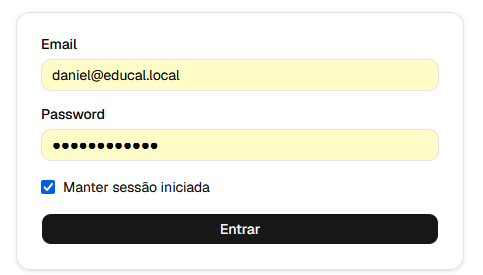
\includegraphics{./figures/app_screenshots/login_interface.png}}
\end{center}
\caption{Login interface.}\label{fig:login}
\end{figure}
\FloatBarrier

\subsection{Calendar Interface} \label{sec:frontend-calendar-ui}
The interactive calendar (Figure~\ref{fig:calendar}) is the core of the application. Its header is split into two rows: a top row with a ``Today'' shortcut and a date navigator (showing the current month/year, an event-count badge for the visible period, and previous/next controls), and an actions row containing the category filter, the Agenda/Day/Week/Month/Year view switcher, the academic-year tools (Section~\ref{sec:frontend-academic-year-tools}), a user filter, the ``Add Event'' button, and the settings menu.

The five views (\textbf{Agenda}, \textbf{Day}, \textbf{Week}, \textbf{Month}, \textbf{Year}; the latter shown in Figure~\ref{fig:calendar}, the rest in Appendix~\ref{app:calendar-views}) offer different levels of temporal density, from a scrollable list grouped by date or category (Agenda) to a full-year grid overview (Year). Within the day/week grid views, occurrences can be rescheduled directly by dragging them to a different time slot, or resized to change their duration, both implemented with the native HTML5 drag-and-drop API and animated with \texttt{framer-motion}; both actions persist immediately through the mutation flow described in Section~\ref{sec:frontend-api}. When a month-view day has more occurrences than can be shown inline, an ``+N more'' control opens a simple list dialog for that day, from which any occurrence can be opened in full detail.

The \texttt{DraggableEvent} component wraps every occurrence block shown in the day and week views, connecting the browser's native drag events to the shared drag-and-drop context (full source in Appendix~\ref{app:draggable-event}, Listing~\ref{lst:draggable-event-full}). It falls back to rendering its children unwrapped, with no drag handlers, for users without editing rights (\texttt{canEditEvents}); otherwise a native \texttt{draggable} \texttt{motion.div} dims itself while being dragged and notifies a shared drag context via \texttt{onDragStart}/\texttt{onDragEnd}. The drop target and resulting date/time update are handled by the companion \texttt{DroppableArea} component and the \texttt{updateOccurrence} mutation (Section~\ref{sec:frontend-api}).

Two controls narrow down what is shown: a category filter (multi-select dropdown, one entry per \texttt{Category}, each with its colored dot) and a user filter (single-select, showing every user's avatar and name, defaulting to ``All users''). A settings menu offers independent toggles for dark/light theme, category badge style (colored block vs. small dot), 12/24-hour time format, and how the Agenda view groups events (by date or by category), all persisted locally per browser.

\begin{figure}[htbp]
\begin{center}
\resizebox{\textwidth}{!}{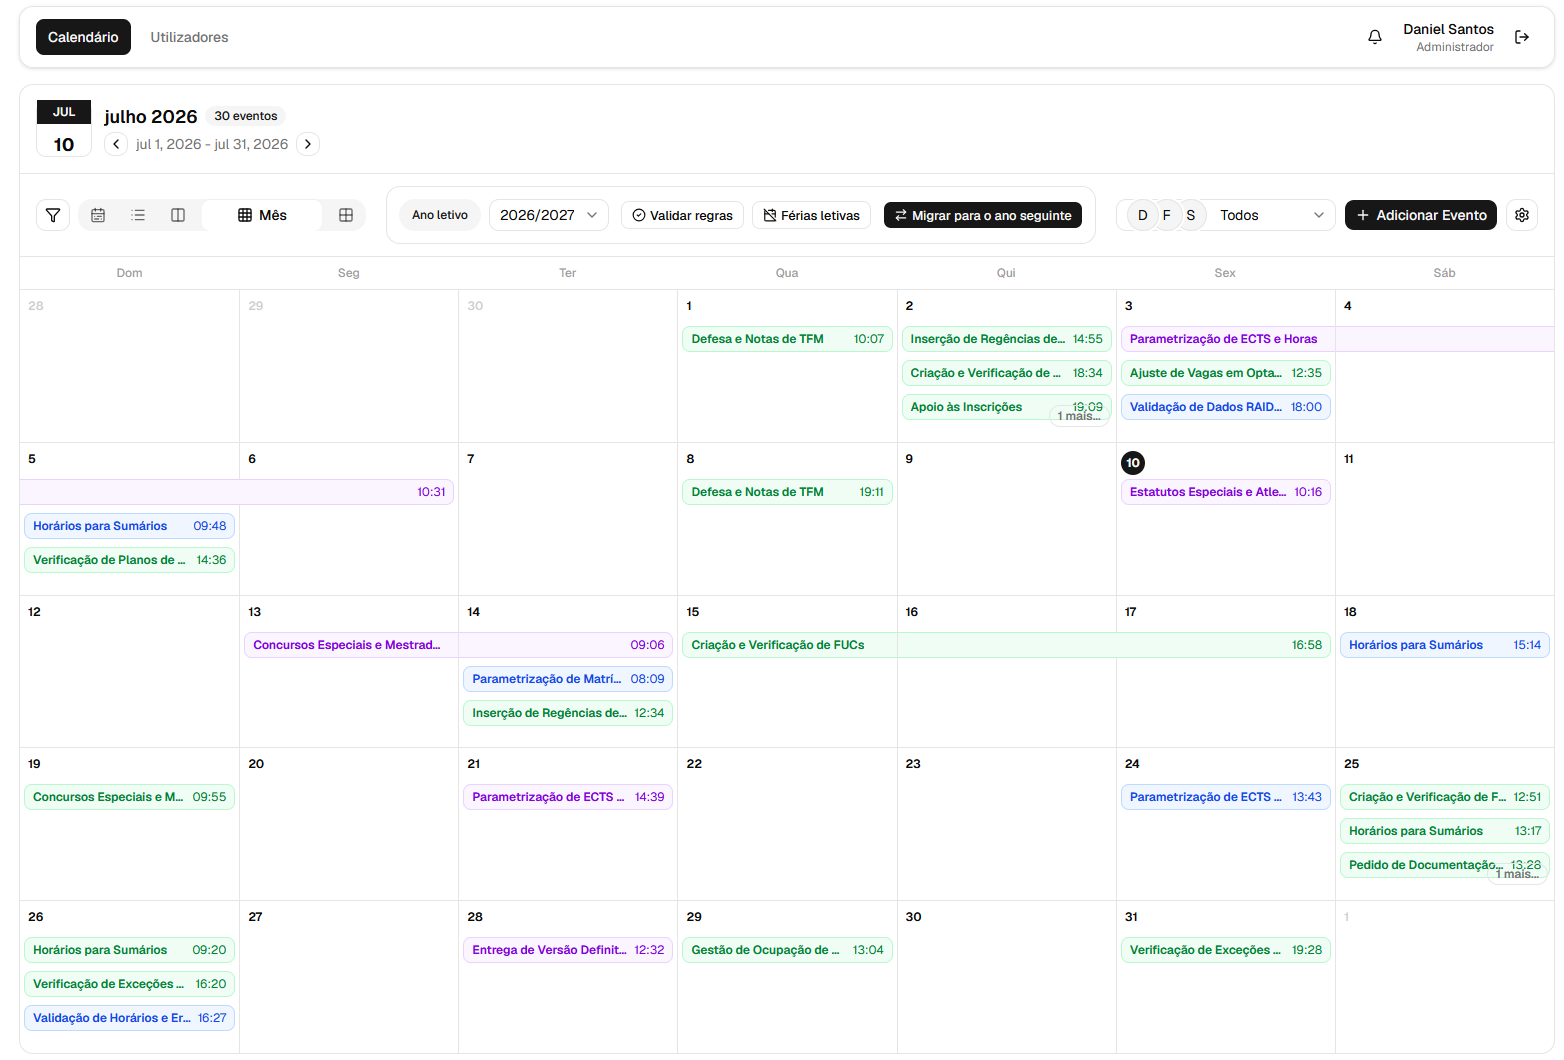
\includegraphics{./figures/app_screenshots/calendar_View.png}}
\end{center}
\caption{Main calendar interface (Month view).}\label{fig:calendar}
\end{figure}
\FloatBarrier

\subsection{Event Management Dialogs} \label{sec:frontend-event-dialogs}
The \textbf{Add/Edit Event dialog} (Figure~\ref{fig:add-edit-event}) is a single form reused for both creating and editing an event, visible only to editors and above. It has an event-level panel (\texttt{name}, \texttt{objective}, \texttt{category}/\texttt{classification}/\texttt{status}/\texttt{responsible} dropdowns, and a default notification lead time, \texttt{notifyDaysBefore}, Section~\ref{sec:backend-notifications}); an occurrence panel, a repeatable list (at least one required) each with its own \texttt{description}, \texttt{start}/\texttt{end date-time}, optional min-duration/min-gap constraints, and its own lead-time override (\texttt{notifyDaysBeforeOverride}); and a ``Rules'' panel attaching any of the five configurable business rules (Section~\ref{sec:rule-engine}), each rendering its own input controls from that rule's field metadata.

\begin{figure}[htbp]
\begin{center}
\resizebox{\textwidth}{!}{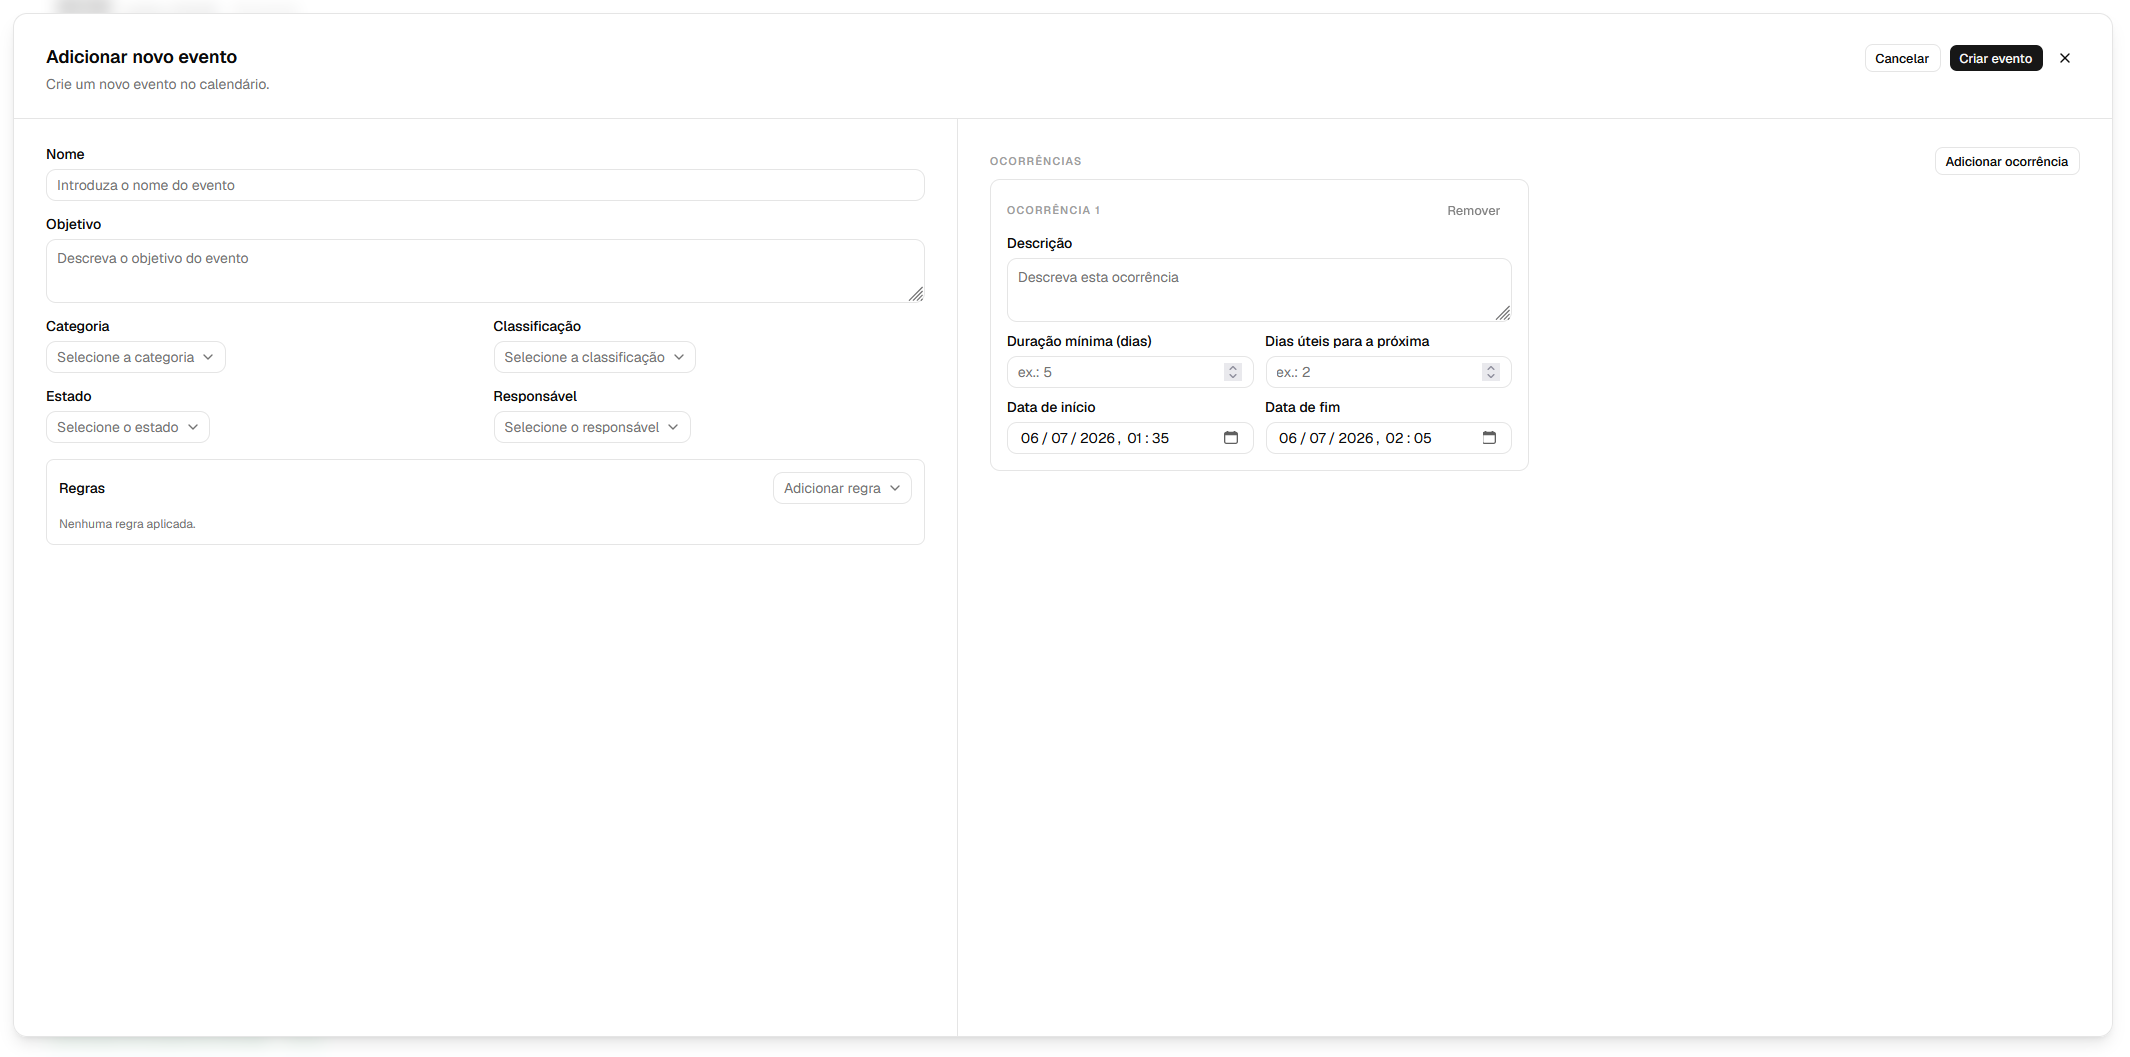
\includegraphics{./figures/app_screenshots/add_edit_event.png}}
\end{center}
\caption{Add/Edit Event dialog.}\label{fig:add-edit-event}
\end{figure}
\FloatBarrier

The \textbf{Event Details dialog} (Figure~\ref{fig:event-details}) is the read-only counterpart, opened when a user clicks an occurrence anywhere in the calendar. It shows the event's name, category/classification/status badges, its objective, who created it, the selected occurrence's dates, every occurrence in a scrollable grid, and a summary of the rules attached to the event, in the same terms an end user configured them in. Users with edit rights see shortcuts here to open the Edit dialog or delete the event directly.

\begin{figure}[htbp]
\begin{center}
\resizebox{\textwidth}{!}{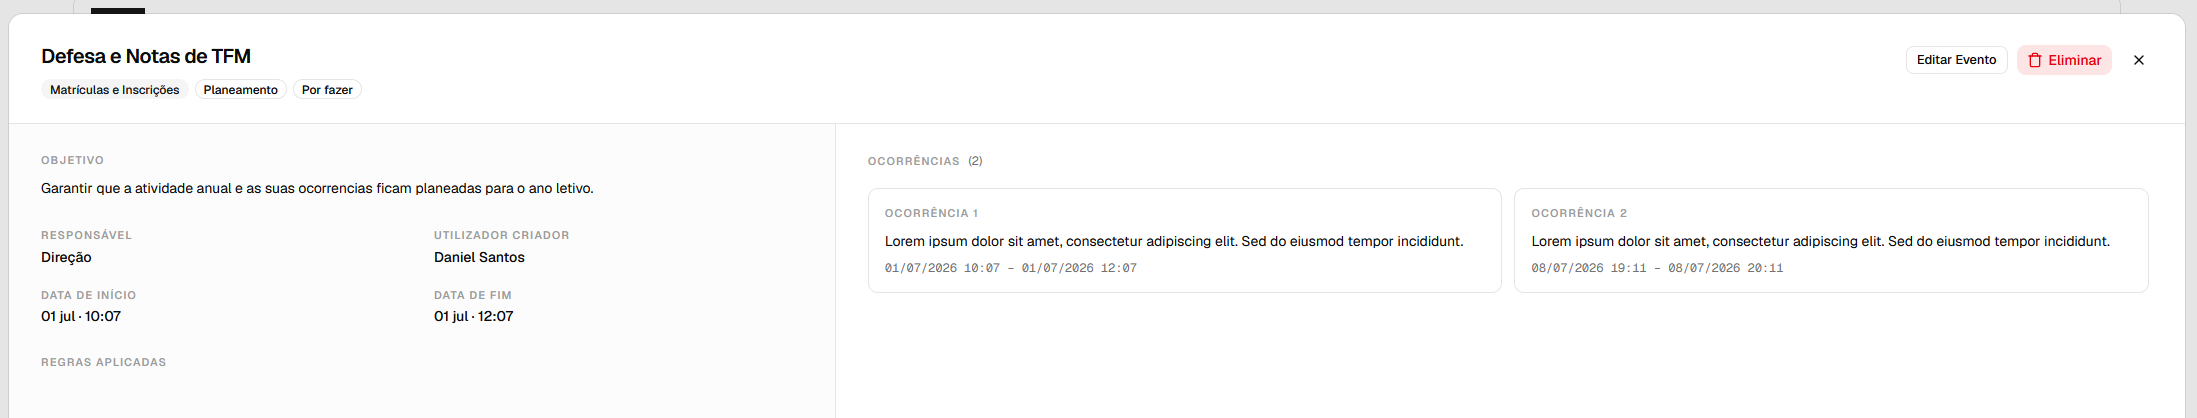
\includegraphics{./figures/app_screenshots/event_details.png}}
\end{center}
\caption{Event Details dialog.}\label{fig:event-details}
\end{figure}
\FloatBarrier

Deleting an event goes through a dedicated \textbf{confirmation dialog} (a destructive-styled button that opens an alert requiring explicit confirmation) before the event and all of its occurrences are removed, since occurrence deletion cascades from the event at the database level (Section~\ref{sec:data-model}).

\subsection{Academic Year Tools} \label{sec:frontend-academic-year-tools}
The academic-year tools, part of the calendar's actions bar, let the user pick an academic year and run the migration workflow described in Section~\ref{sec:migration-engine}: ``Validate'' checks the selected year's events against every business rule without changing anything, and ``Migrate'' (editors and administrators only) runs the full migration. Both share a results modal (Appendix~\ref{app:screenshots}, Figure~\ref{fig:migration-report-full}): a confirmation banner if no violations were found, or one card per violation otherwise, naming the rule, the affected event/occurrence, and the offending date, opening that event's Details dialog on click. A separate ``Vacations'' action opens a dedicated dialog (Figure~\ref{fig:vacations}) for managing that year's vacation periods, with full create/edit/delete support for editors.

\begin{figure}[htbp]
\begin{center}
\resizebox{90mm}{!}{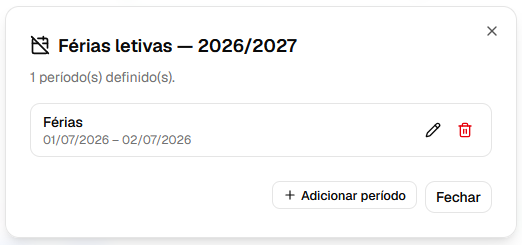
\includegraphics{./figures/app_screenshots/vacations_dialog.png}}
\end{center}
\caption{Vacation periods dialog.}\label{fig:vacations}
\end{figure}
\FloatBarrier

\subsection{User Management Dashboard} \label{sec:frontend-user-mgmt}
The administrative dashboard (Figure~\ref{fig:user-mgmt}), accessible only to administrators, lists every user in a table (name, email, role, profile picture, and actions) and supports full CRUD, with the password field left blank on edit meaning ``keep the current password''. Every mutation gives immediate toast feedback, deletions are confirmed before proceeding, and the delete action is disabled for the currently logged-in administrator's own row, reinforcing the ``cannot delete self'' invariant already enforced on the backend (Section~\ref{sec:backend-rbac}).

\begin{figure}[htbp]
\begin{center}
\resizebox{\textwidth}{!}{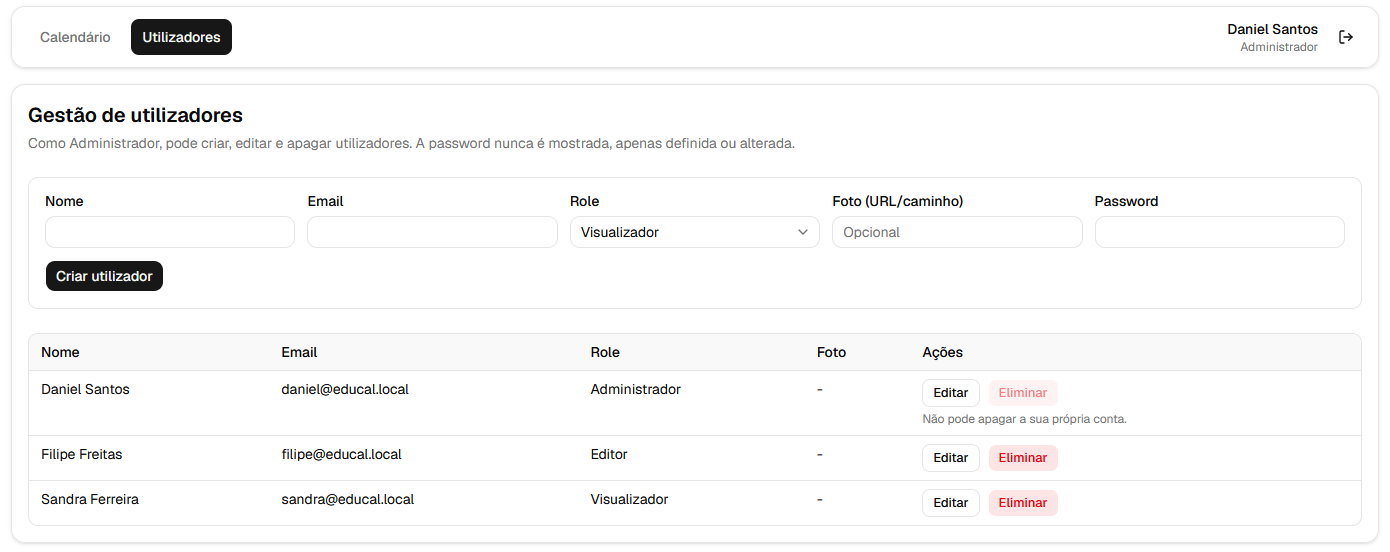
\includegraphics{./figures/app_screenshots/user_management.png}}
\end{center}
\caption{User management dashboard.}\label{fig:user-mgmt}
\end{figure}
\FloatBarrier
